% Created 2018-12-16 do. 20:45
% Intended LaTeX compiler: pdflatex
\documentclass[xcolor={usenames,svgnames,dvipsnames}]{beamer}
\usepackage[utf8]{inputenc}
\usepackage[T1]{fontenc}
\usepackage{graphicx}
\usepackage{grffile}
\usepackage{longtable}
\usepackage{wrapfig}
\usepackage{rotating}
\usepackage[normalem]{ulem}
\usepackage{amsmath}
\usepackage{textcomp}
\usepackage{amssymb}
\usepackage{capt-of}
\usepackage{hyperref}
\usepackage{color}
\usepackage{listings}
\usepackage{mathpazo}
\usepackage{gensymb}
\usepackage{amsmath}
\usepackage{chemarr}%flechas para reacciones químicas (SFER.tex)
\bibliographystyle{plain}
\AtBeginSubsection[]{\begin{frame}[plain]\tableofcontents[currentsubsection,sectionstyle=show/shaded,subsectionstyle=show/shaded/hide]\end{frame}}
\AtBeginSection[]{\begin{frame}[plain]\tableofcontents[currentsection,hideallsubsections]\end{frame}}
\usepackage[emulate=units]{siunitx}
\sisetup{fraction=nice, decimalsymbol=comma, retain-unity-mantissa = false}
\newunit{\wattpeak}{Wp}
\newunit{\watthour}{Wh}
\newunit{\amperehour}{Ah}
\usepackage{steinmetz}
\hypersetup{colorlinks=true, linkcolor=Blue, urlcolor=Blue}
\renewcommand{\thefootnote}{\fnsymbol{footnote}}
\beamertemplatenavigationsymbolsempty
\setbeamertemplate{footline}[frame number]
\setbeamercolor{alerted text}{fg=blue!50!black} \setbeamerfont{alerted text}{series=\bfseries}
\usetheme[hideothersubsections]{Goettingen}
\usecolortheme{rose}
\usefonttheme{serif}
\author{Oscar Perpiñán Lamigueiro}
\date{\url{http://oscarperpinan.github.io}}
\title{Sistemas Fotovoltaicos de Bombeo}
\subtitle{Conceptos Generales y Componentes}
\hypersetup{
 pdfauthor={Oscar Perpiñán Lamigueiro},
 pdftitle={Sistemas Fotovoltaicos de Bombeo},
 pdfkeywords={},
 pdfsubject={},
 pdfcreator={Emacs 26.1 (Org mode 9.1.14)}, 
 pdflang={Spanish}}
\begin{document}

\maketitle

\section{Introducción}
\label{sec:orgd85839c}

\begin{frame}[label={sec:orgd66dd59}]{Agua y ESF}
\begin{itemize}
\item Las \alert{curvas de generación fotovoltaica y de consumo de agua están bien adaptadas}: las épocas de mayor calor y radiación solar son de mayor consumo de agua.

\item Se puede utilizar el \alert{agua como medio de acumulación de energía}, evitando baterías con el consiguiente ahorro de costes, a la vez que aumenta la seguridad, eficiencia y fiabilidad.

\item El bombeo de agua directo fotovoltaico es limpio: \alert{no presenta los riesgos de una contaminación del pozo a causa de posibles derrames de combustible}. Asimismo, se evitan los problemas logísticos de suministro y transporte de carburante.
\end{itemize}
\end{frame}


\begin{frame}[label={sec:org9ee7140}]{Composición}
\begin{center}
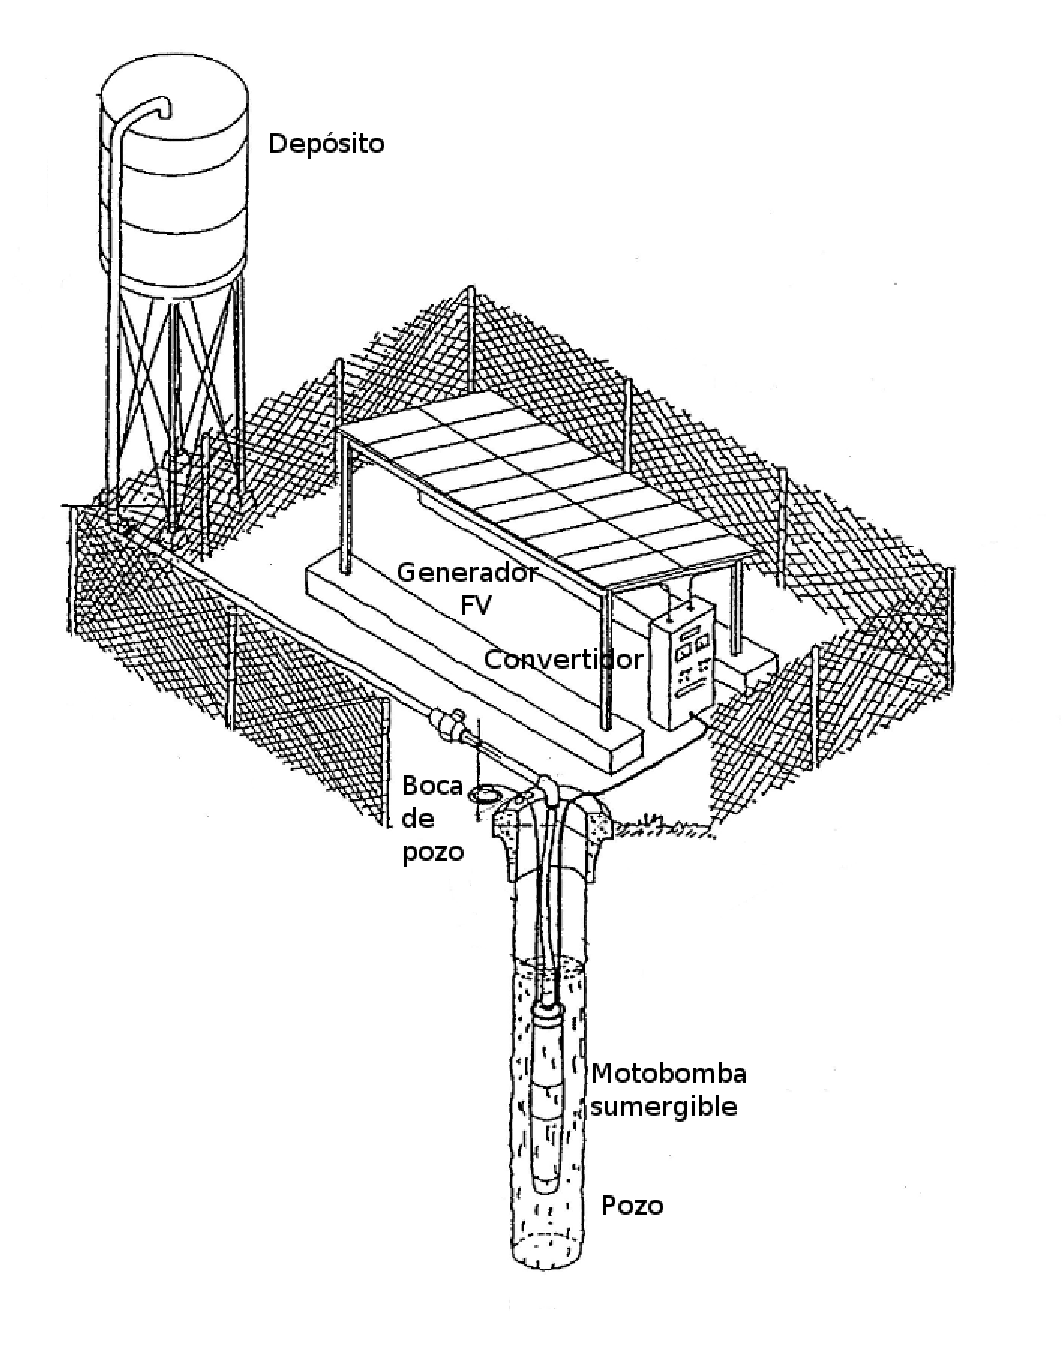
\includegraphics[height=\textheight]{../figs/EsquemaBombeo_oscar.pdf}
\end{center}
\end{frame}

\section{Motobombas}
\label{sec:orgb5d52d7}

\begin{frame}[label={sec:orgb7b6d83}]{Definición}
\begin{block}{Motor eléctrico}
Máquina eléctrica que \alert{transforma energía eléctrica en energía mecánica} por medio de interacciones electromagnéticas.
\end{block}

\begin{block}{Bomba}
\alert{Máquina hidráulica} generadora que \alert{transforma la energía mecánica} con la que es accionada \alert{en energía hidráulica del fluido} (agua).
\end{block}
\end{frame}

\subsection{Motores eléctricos en ESF}
\label{sec:orgf4fffff}

\begin{frame}[label={sec:org2cc1da1}]{Motor DC}
\begin{itemize}
\item \alert{Estator-Inductor} alimentado por \alert{corriente DC} (o imanes permanentes).

\item El \alert{colector de delgas} transforma la frecuencia de alimentación (DC) en alterna.

\item \alert{Rotor-Inducido gira sincronizado} con la frecuencia \guillemotleft{}transformada\guillemotright{}.

\item Los \alert{motores DC con escobillas están sometidos a desgaste}. Necesitan mantenimiento y por tanto deben evitarse con bombas sumergidas.

\item Existen \alert{motores DC sin escobillas}, donde la conmutación se realiza mediante un \alert{circuito electrónico}.

\item No necesitan inversor (pero si \alert{adaptador}), tienen buen rendimiento, pero están indicados para \alert{potencias bajas}.
\end{itemize}
\end{frame}

\begin{frame}[label={sec:org20d21a6}]{Motor asíncrono o de inducción}
\begin{itemize}
\item \alert{Estator-inductor} alimentado por una \alert{corriente trifásica alterna}.  Produce un campo giratorio.

\item \alert{Rotor-inducido} constituido por \alert{espiras cortocircuitadas} (jaula de ardilla).

\item Son los más comunes, y más baratos que los DC.

\item Tienen \alert{pares de arranque muy bajos}, adecuados para bombas que requieren bajo par de arranque, como las \alert{centrífugas}.
\end{itemize}
\end{frame}

\subsection{Bombas}
\label{sec:org153985b}

\begin{frame}[label={sec:org0075695}]{Ecuación de Bernouilli}
\begin{block}{Conservación de energía}
$$\frac{\Delta p}{\rho}+\frac{\Delta v^2}{2}+g\cdot\Delta h=cte.$$
\begin{itemize}
\item \(\Delta p\): presión (bombas de desplazamiento positivo)
\item \(\Delta v^2\): velocidad (bombas rotodinámicas)
\item \(\Delta h\): altura (objetivo)
\end{itemize}
\end{block}
\end{frame}


\begin{frame}[label={sec:org7f8c7d6}]{Bombas de desplazamiento positivo}
\[
\frac{\Delta p}{\rho}+\frac{\Delta v^2}{2}+g\cdot\Delta h=cte.
\]

\begin{block}{\alert{Principio}: cambio de presión}
El aumento de presión se realiza por el empuje de las paredes de las cámaras que varían su volumen.
\end{block}
\end{frame}

\begin{frame}[label={sec:org1e73092}]{Bombas de membrana}
\alert{Bombas oscilantes}, compartimentos fijos de volumen variable por el movimiento de un pistón o por la deformación de un diafragma.
\begin{center}
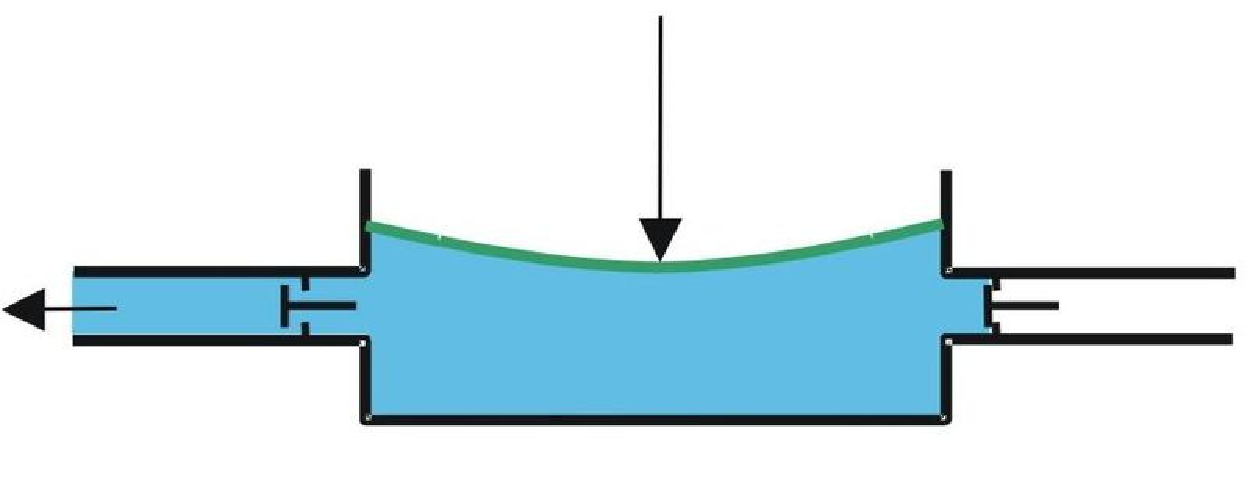
\includegraphics[height=0.3\textheight]{../figs/800px-Bomba_diafragma_impulsando.pdf}
\end{center}
\begin{center}
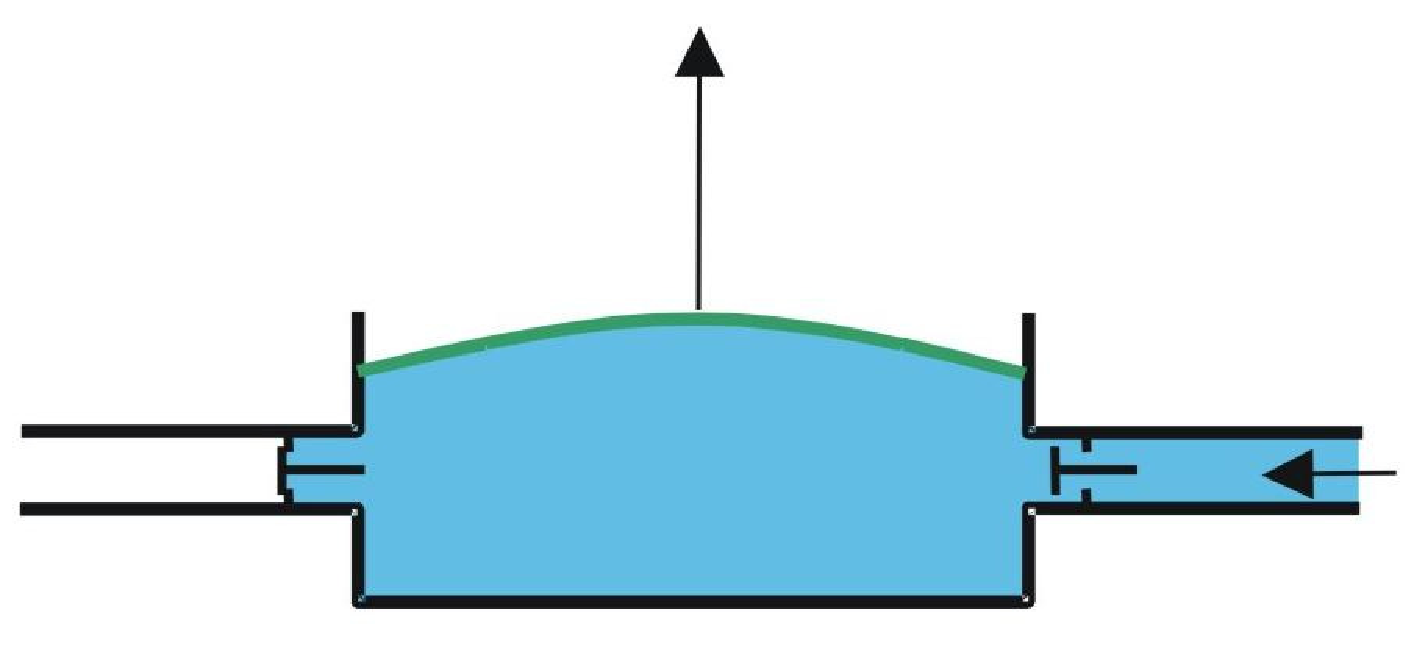
\includegraphics[height=0.3\textheight]{../figs/Bomba_diafragma_aspirando.pdf}
\end{center}
\end{frame}

\begin{frame}[label={sec:org8aa52c8}]{Bombas helicoidales}
\alert{Bombas rotatorias}, compartimentos que se desplazan desde la zona de entrada (de baja presión) hasta la zona de salida (de alta presión) de la máquina. (p.ej. bomba de tornillo o helicoidal).

\begin{center}
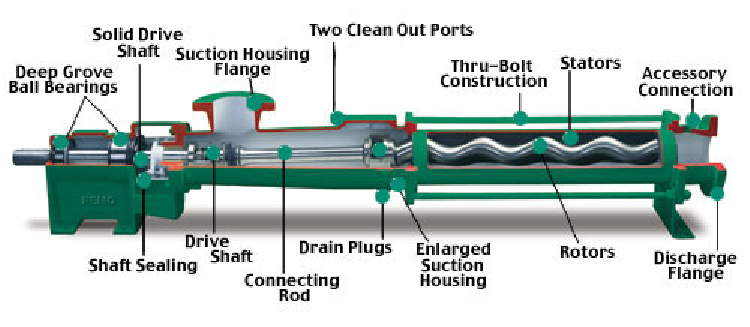
\includegraphics[width=.9\linewidth]{../figs/bombatornillo.pdf}
\end{center}
\end{frame}

\begin{frame}[label={sec:orgf82a0cd}]{Bombas helicoidales y de membrana}
\begin{itemize}
\item Son apropiadas para \alert{altos incrementos de presión y bajos caudales}.

\item Necesitan un \alert{elevado par de arranque} (por tanto no pueden ser acopladas directamente al generador).

\item Las bombas de diafragma, más económicas, requieren el \alert{reemplazo de los diafragmas} cada dos o tres años, dependiendo del fabricante.
\end{itemize}
\end{frame}

\begin{frame}[label={sec:org26cfe8f}]{Bombas rotodinámicas}
\[
\frac{\Delta p}{\rho}+\frac{\Delta v^2}{2}+g\cdot\Delta h=cte.
\]

\begin{block}{\alert{Principio}: añadir cantidad de movimiento}
En este tipo de bombas hay uno o varios rodetes con álabes que giran generando un campo de presiones en el fluido.
\end{block}
\end{frame}

\begin{frame}[label={sec:orgc93d13d}]{Bombas centrífugas}
\begin{itemize}
\item El fluido entra por el centro del rodete cuyos álabes conducen el fluido

\item Por la fuerza centrífuga es impulsado hacia el exterior y es recogido por la carcasa

\item Es conducido hacia la salida o hacia el siguiente rodete (bombas multietapa)
\end{itemize}

\begin{center}
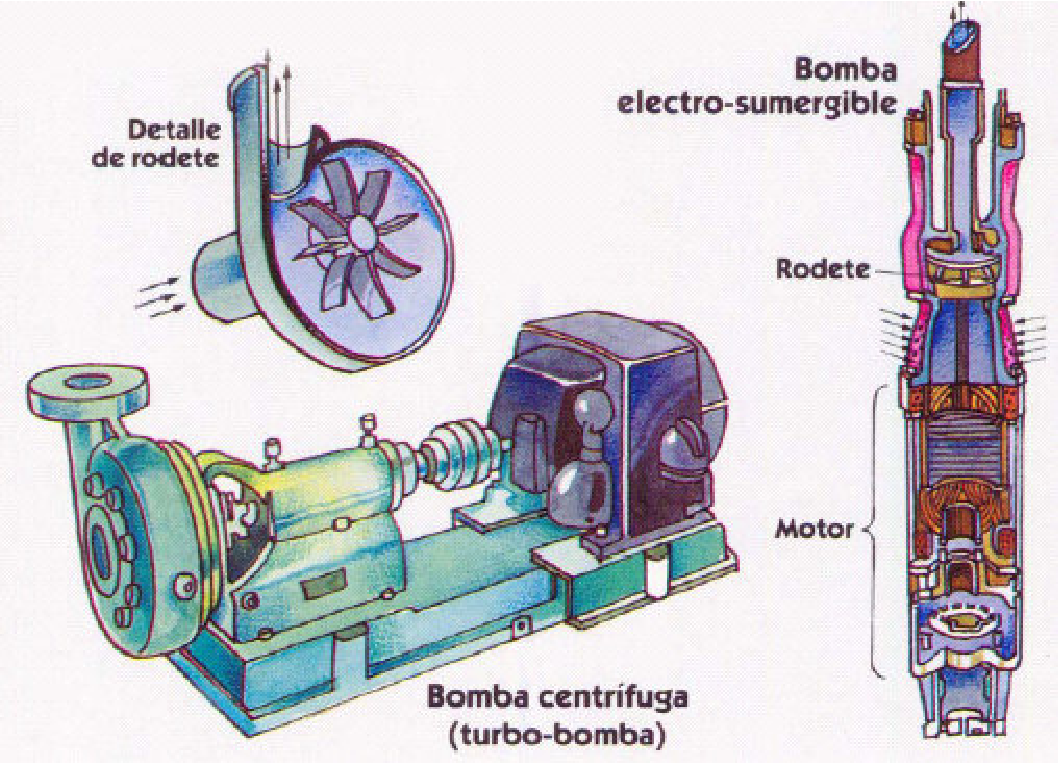
\includegraphics[height=0.5\textheight]{../figs/BombaCentrifuga.pdf}
\end{center}
\end{frame}

\begin{frame}[label={sec:org7e8d47f}]{Bombas centrífugas}
\begin{itemize}
\item Están diseñadas para vencer una \alert{presión más o menos constante},

\item Proporcionan \alert{elevados caudales para bajas alturas manométricas}.

\item Se puede aumentar la altura añadiendo etapas en serie en la misma bomba (bomba multietapa)

\item Son \alert{bombas simples y robustas, de bajo coste}.

\item Funcionan bien con pequeños pares de arranque.
\end{itemize}
\end{frame}


\begin{frame}[label={sec:org7f67cfa}]{Según la disposición}
\begin{itemize}
\item \alert{Bombas sumergibles}

\begin{itemize}
\item Pozos profundos de pequeño diámetro

\item Normalmente ensambladas con el motor.
\end{itemize}

\item \alert{Bombas flotantes}

\begin{itemize}
\item Instalación en ríos, lagos o pozos de gran diámetro en flotación.

\item Mucho caudal pero poca altura manométrica
\end{itemize}

\item \alert{Bombas de superficie}

\begin{itemize}
\item Instaladas a nivel de suelo (fácil mantenimiento)

\item Tienen un límite en el nivel de succión (8 metros).

\item Si utilizan agua como lubricante, no deben operar en seco para evitar el sobrecalentamiento.
\end{itemize}
\end{itemize}
\end{frame}

\begin{frame}[label={sec:org52f9532}]{Configuraciones típicas}
\begin{itemize}
\item \alert{Sistemas de baja potencia (50 a 400 Wp)}

\begin{itemize}
\item Motor DC accionando una bomba de membrana
\end{itemize}

\item \alert{Sistemas de media potencia (400-1500 Wp)}

\begin{itemize}
\item Bomba sumergible centrífuga multietapa con motor asíncrono

\item Motor DC sin escobillas accionando una bomba helicoidal
\end{itemize}

\item \alert{Potencia superior a 1 kWp}

\begin{itemize}
\item Bomba sumergible centrífuga multietapa con motor asíncrono
\end{itemize}
\end{itemize}
\end{frame}
\section{Acoplamiento generador-motobomba}
\label{sec:org8da5f97}


\begin{frame}[plain,label={sec:orgbed4c59}]{Motivo}
\begin{columns}
\begin{column}{0.8\columnwidth}
\begin{itemize}
\item La \alert{potencia y tensión suministrada por un generador FV varían} con la radiación y la temperatura.

\item Las condiciones de funcionamiento \alert{no se adaptan siempre a todos los requerimientos de la motobomba}.

\item Es necesario adaptar las condiciones de funcionamiento de la motobomba al punto de trabajo del generador FV.

\begin{itemize}
\item \alert{Motor AC: variador de frecuencia}

\item \alert{Motor DC: convertidor DC-DC}
\end{itemize}
\end{itemize}
\end{column}

\begin{column}{0.4\columnwidth}
\begin{center}
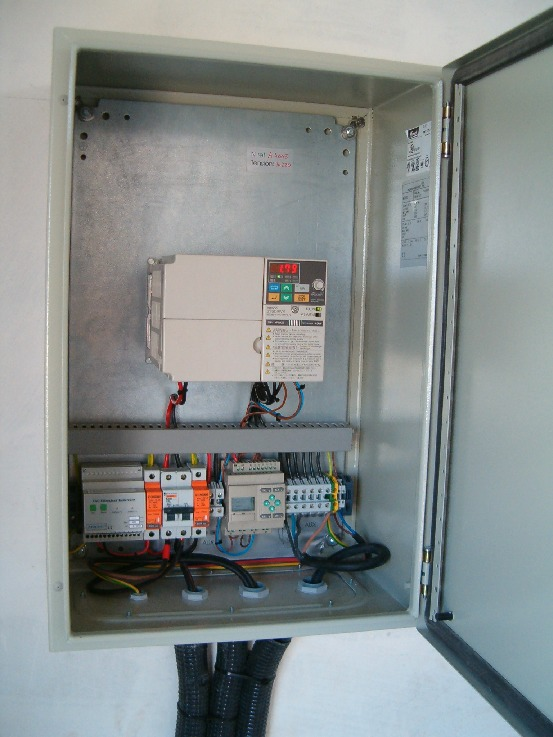
\includegraphics[width=.9\linewidth]{../figs/VariadorFrecuencia.jpg}
\end{center}
\end{column}
\end{columns}
\end{frame}

\subsection{Convertidores}
\label{sec:org2811427}
\begin{frame}[label={sec:org837c42b}]{Convertidor DC-DC}
\begin{itemize}
\item Dispositivo que \alert{transforma corriente continua de una tensión a otra}.

\begin{itemize}
\item Suelen ser reguladores de conmutación, dando a su salida una tensión regulada.
\end{itemize}

\item Se utiliza para alimentar \alert{motores DC con generador FV}.

\item Normalmente no incorporan buscador de MPP.
\end{itemize}
\end{frame}

\begin{frame}[label={sec:orgdc8af02}]{Variador de frecuencia}
\begin{itemize}
\item El variador de frecuencia \alert{transforma una señal alterna de una frecuencia en otra señal alterna de otra frecuencia}.

\item Está compuesto por un rectificador y un inversor con frecuencia variable.

\item Eficiencia cercana al 95\%.

\item Habitualmente sin seguidor de MPP.
\end{itemize}

\begin{center}
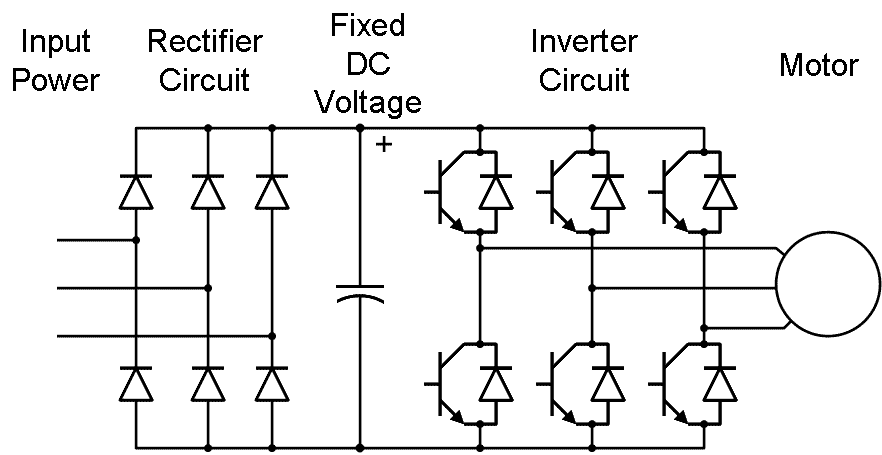
\includegraphics[width=.9\linewidth]{../figs/VariadorFrecuencia_esquema.png}
\end{center}
\end{frame}


\subsection{Protecciones}
\label{sec:orgd3ededb}

\begin{frame}[label={sec:orgddef6f4}]{Pozo vacío}
\begin{block}{Control de frecuencia de salida del variador}
\begin{itemize}
\item Cuando el motor trabaja en vacío, la corriente consumida baja y el variador debe subir la frecuencia para alcanzar la tensión de referencia.

\item Si se supera la frecuencia de 55 Hz se para el sistema y se marca un intervalo de espera para permitir que el pozo vuelva a llenarse.
\end{itemize}
\end{block}
\end{frame}

\begin{frame}[label={sec:org7a35c2c}]{Deposito lleno}
\begin{block}{Presostáto en la tubería combinado con una boya en el depósito}
\begin{itemize}
\item Cuando en el depósito se alcanza un nivel determinado, la boya acciona el cierre de la entrada al depósito.

\item Sin embargo, la bomba sigue elevando agua. De esta forma, la presión dentro de la tubería aumenta hasta accionar el presostato.

\item Se pone en marcha un temporizador para permitir que baje el nivel del depósito.
\end{itemize}
\end{block}
\end{frame}


\section{Circuito Hidráulico}
\label{sec:org01f425b}

\begin{frame}[plain,label={sec:org4613b25}]{Circuito hidráulico}
\begin{columns}
\begin{column}{0.5\columnwidth}
\begin{itemize}
\item Tubería de impulsión

\item Boca de pozo

\item Tubería de distribución y valvulería
\end{itemize}
\end{column}

\begin{column}{0.6\columnwidth}
\begin{center}
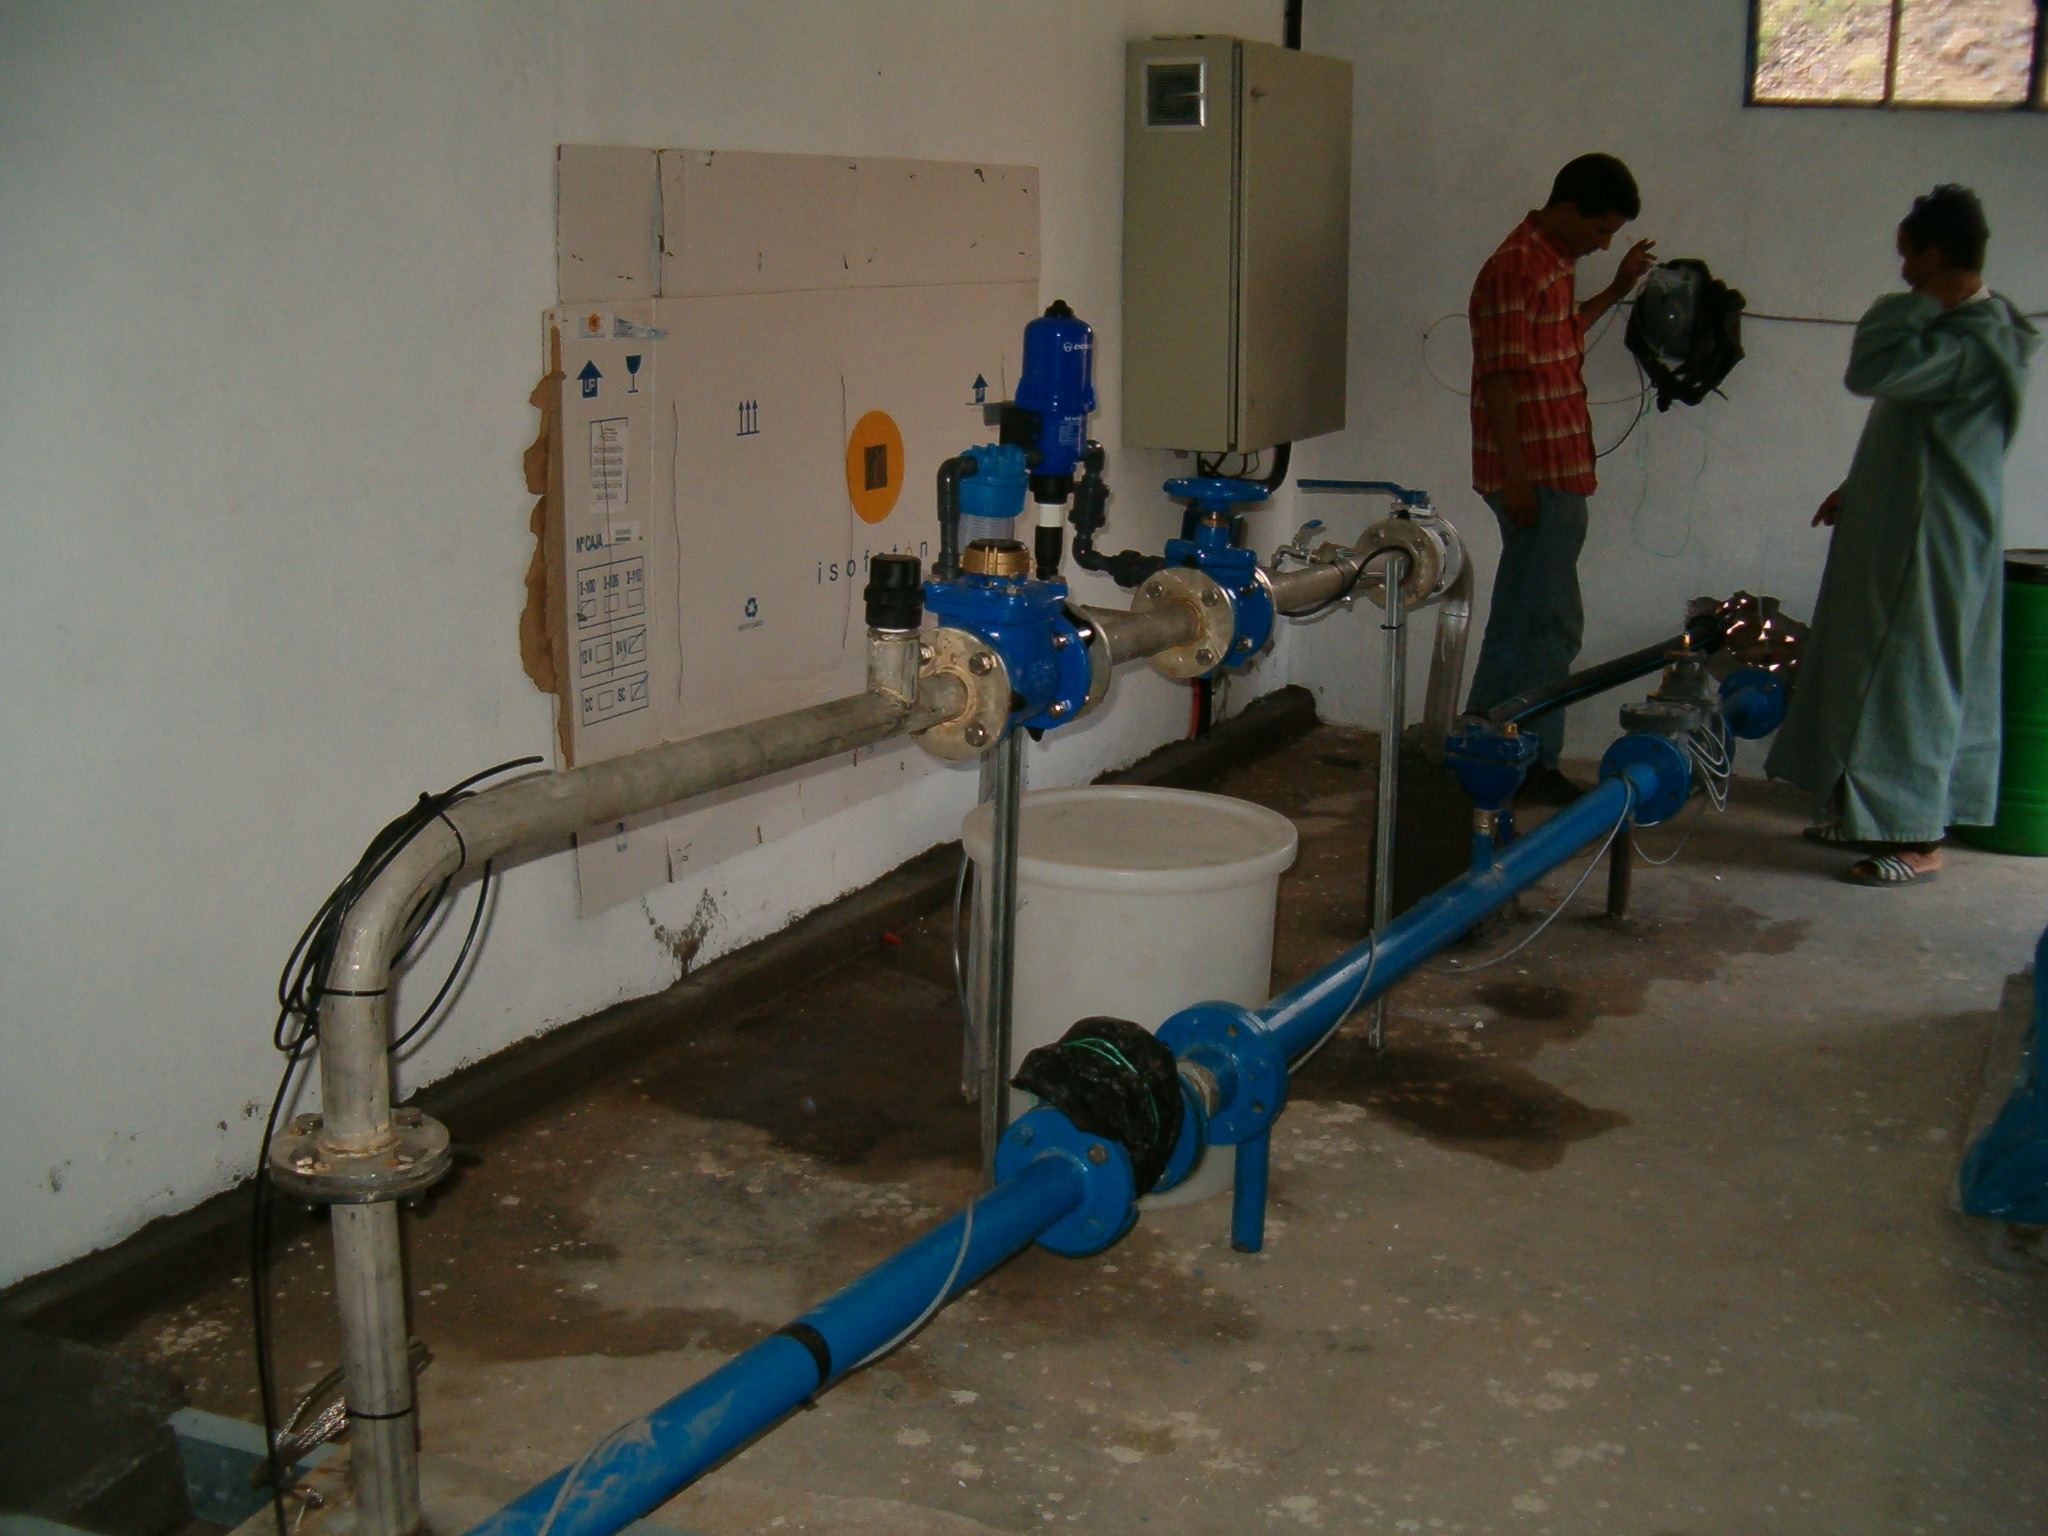
\includegraphics[width=.9\linewidth]{../figs/CircuitoHidraulico.jpg}
\end{center}
\end{column}
\end{columns}
\end{frame}


\begin{frame}[plain,label={sec:orgffeafc3}]{Tubería de Impulsión}
\alert{Tubería instalada a la salida de la bomba.}

\begin{columns}
\begin{column}{0.6\columnwidth}
\begin{itemize}
\item Polietileno de alta densidad y calidad alimentaria

\begin{itemize}
\item Coste menor

\item Tendencia a enrollarse.
\end{itemize}

\item Tuberías autoportantes flexibles

\begin{itemize}
\item Coste mayor

\item Requiere terminales específicos fabricados en acero inoxidable
\end{itemize}
\end{itemize}
\end{column}
\begin{column}{0.6\columnwidth}
\begin{center}
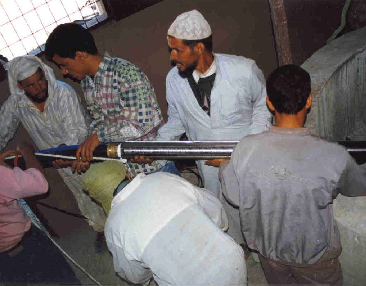
\includegraphics[width=.9\linewidth]{../figs/Marruecos4.png}
\end{center}
\end{column}
\end{columns}
\end{frame}


\begin{frame}[plain,label={sec:orga807cf6}]{Depósito elevado}
\begin{columns}
\begin{column}{0.6\columnwidth}
\begin{itemize}
\item \alert{Tamaño adecuado para 1 o 2 días de consumo}
\item Para depósitos pequeños (20 a 1.000 l) debe elegirse un \alert{depósito plástico de color negro}  para evitar aparición de algas y otros contaminantes.
\end{itemize}
\end{column}

\begin{column}{0.6\columnwidth}
\begin{center}
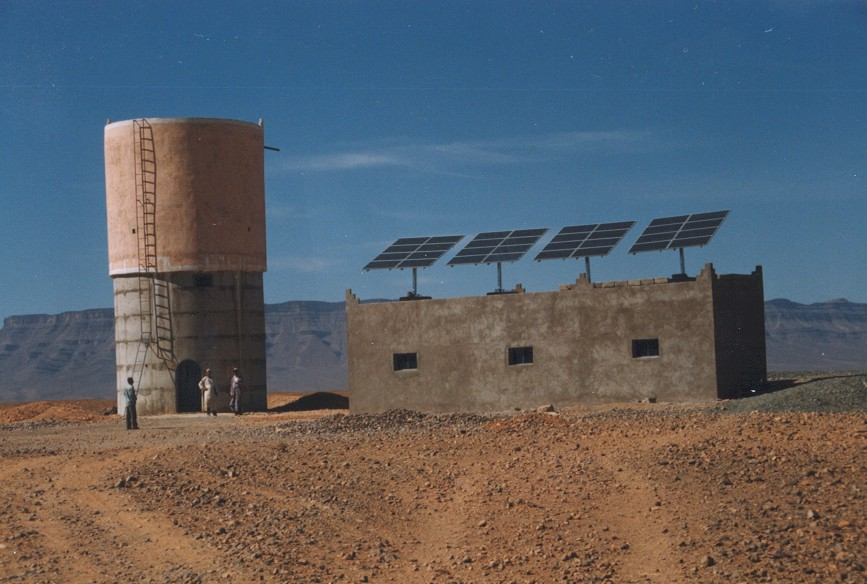
\includegraphics[width=.9\linewidth]{../figs/Bombeo.jpg}
\end{center}
\end{column}
\end{columns}
\end{frame}
\end{document}